% ---------------------------------------------------------------------
% HEADER
% Formålet med å legge header til et eget dokument er å garantere at
% oppsettet av dokumentene er likt for alle løsningsforslagene.
% I headeren skjer følgende:
% (1) Dokumentet blir startet
% (2) Pakker blir importert
% ---------------------------------------------------------------------
\input{../../header.tex}


% ---------------------------------------------------------------------
% DOKUMENTVARIABLER
% ---------------------------------------------------------------------
\newcommand{\fagkode}{R1}
\newcommand{\semesteraar}{våren 2018}
\newcommand{\forfatter}{Anita G.}
\newcommand{\dokumenttittel}{Løsningsforslag -- Eksamen \fagkode, \semesteraar}

\usepackage{siunitx}


% Set til 'true' og oppgi logo dersom du vil bruke en logo
\newboolean{bruklogo}
\setboolean{bruklogo}{false}
\newcommand{\logonavn}{}



% ---------------------------------------------------------------------
% SETUP
% Formålet med å legge setup til et eget dokument å garantere at headers,
% footers, og øverste del av dokumentet er likt for alle
% løsningsforslagene.
% ---------------------------------------------------------------------
\input{../../setup.tex}


% ---------------------------------------------------------------------
% DOKUMENTSTART - Skriv løsningsforslaget nedenfor
% ---------------------------------------------------------------------	
\section*{Del 1 - uten hjelpemidler}
\subsection*{Oppgave 1}
\begin{easylist}[enumerate]
	\ListProperties(Style2*=,Numbers=a,Numbers1=l,FinalMark={)})
	# Vi skal derivere $f(x) = x^4 - x +2$. Vi bruker regelen $f(x) = x^n \Rightarrow f'(x) = nx^{n-1}$. Vi får da at $f'(x) = 4x^3 - 1$.
	
	# Her ser vi at funksjonen g er sammensatt av to funksjoner som er multiplisert sammen, nemlig $x^3$ og $\ln(x)$. Vi bruker derfor produktregelen: $f(x) = uv \Rightarrow f'(x) = u'v + uv'$. Vi får da 
	\begin{equation*}
		\begin{aligned}
			g'(x) &= 3x^2 \cdot \ln(x) + x^3 \cdot \frac{1}{x}\\
					&= 3x^2\ln(x) + x^2\\
					&= x^2(3\ln(x)+1)\\
		\end{aligned}
	\end{equation*}
	
	# Her får vi bruk for kjerneregelen, der vi velger at kjernen vår er $u = 2x^2 + x$. Vi har at 
	\begin{equation*}
		\begin{aligned}
				h(x) = e^{u(x)} \Rightarrow h'(x) &= (e^{u(x)})' \cdot u'(x) \\
																  &= e^{u(x)} \cdot (4x + 1) \\
																  &= (4x +1)e^{2x^2 + x}
		\end{aligned}
	\end{equation*}
\end{easylist}


\subsection*{Oppgave 2}
\begin{easylist}[enumerate]
	\ListProperties(Style2*=,Numbers=a,Numbers1=l,FinalMark={)})
	# 
	\begin{equation*}
		\frac{1}{2x-2} + \frac{2}{x-3} - \frac{x-2}{x^2 - 4x +3}
	\end{equation*}
	Først faktoriserer vi nevnerene for å finne ut hva fellesnevneren til brøkene er. Nevneren i det første leddet faktoriseres slik: $2x-2 = 2(x-1)$. Nevneren i andre legg kan ikke faktoriseres, mens nevneren i det tredje leddet kan vi faktorisere for eksempel ved bruk av abc-formelen. Etter faktoriseringen ser uttrykket ut slik
	
	\begin{equation*}
		\begin{aligned}
			\frac{1}{2(x-1)} + \frac{2}{x-3} - \frac{x-2}{(x-1)(x-3)}
		\end{aligned}
	\end{equation*}
	
	Vi ser dermed at fellesnevneren er $2(x-1)(x-3)$. Vi ganger første ledd med $(x-3)$ i både teller og nevner, andre ledd med $2(x-1)$ og tredje ledd med $2$.
	
	\begin{equation*}
		\begin{aligned}
			&\frac{1(x-3)}{2(x-1)(x-3)} + \frac{2 \cdot 2(x-1)}{2(x-1)(x-3)} - \frac{2(x-3)}{2(x-1)(x-3)} \\
			& = \frac{x - 3 +4x - 4 - 2x + 4}{2(x-1)(x-3)} \\
													& = \frac{3x-3}{2(x-1)(x-3)}\\
													& = \frac{3(x-1)}{2(x-1)(x-3)} \\
													& = \frac{3}{2(x-3)}
		\end{aligned}
	\end{equation*}
	
	# Her må vi ta i bruk logaritmesetningene. Disse er: $\ln(ab) = \ln(a) + \ln(b)$, $\ln\left(\frac{a}{b}\right) = \ln(a) - \ln(b)$ og $\ln(a^x) = x \cdot \ln(a)$.
	\begin{equation*}
		\begin{aligned}
		&2\ln(x\cdot y^3) - \frac{1}{2} \ln \left (\frac{x^4}{y^2} \right) \\
		& = 2(\ln(x) + \ln(y^3) - \frac{1}{2}(\ln(x^4) - \ln(y^2)) \\
		& = 2(\ln(x) + 3\ln(y)) - \frac{1}{2}(4\ln(x) - 2\ln(y))\\
		& = 2\ln(x) + 6\ln(y) - 2\ln(x) + \ln(y)\\
		& = \answer{7\ln(y)}
		\end{aligned}
	\end{equation*}
	
\end{easylist}

\subsection*{Oppgave 3}

\begin{easylist}[enumerate]
	\ListProperties(Style2*=,Numbers=a,Numbers1=l,FinalMark={)})
	# Vektoren mellom to punkter $(x_1,y_1)$ og $(x_2,y_2)$ er gitt ved $[x_2 - x_1, y_2 -y_1]$. Vi får da: \newline
	$\vec{AB} = [-1-(-2), -3-(-1)] = [1,-2]$\newline
	$\vec{BC} = [3-(-1),-1-(-3)] = [4,2]$
	
	# Vi har at de to vektorene står vinkelrett på hverandre dersom $\vec{AB} \cdot \vec{BC} = 0$\newline
	$\vec{AB} \cdot \vec{BC} = [1,-2] \cdot [4,2] = 1 \cdot 4 + (-2) \cdot 2 = 4 + (-4) = 0$
	\newline \newline
	Vektorene står vinkelrett på hverandre.
	
	# Vektorene $\vec{CD}$ og $\vec{AB}$ er parallelle dersom $\vec{CD} = k \cdot \vec{AB}$ der $k$ er et tall. Vi finner først $\vec{CD}$ på samme måte som vi fant vektorene i oppgave a. \newline
	$\vec{CD} = [t-3,t^2 + 2- (-1)] = [t-3,t^2 + 3]$\newline \newline
	\begin{equation*}
		\begin{aligned}
		\vec{CD} & = k \cdot \vec{AB}\\
		[t-3,t^2 + 3] & = k \cdot [1,-2] &  = [k,-2k]\\
		\end{aligned}
	\end{equation*}
	
	For at to vektorer skal være like må x-koordinatene være like hverandre og y-koordinatene være like hverandre i de to vektorene. Vi får altså to likninger med to ukjente: 
	
	\begin{equation*}
		\begin{aligned}
		t-3 = k &\:\:\: \vee & t^2 + 3 = -2k \\
		\end{aligned}
	\end{equation*}
	
	Likning nr 1 gir oss et uttrykk for $k$. Dette setter vi inn for $k$ i likning nr 2 og løser for $t$.
	
	\begin{equation*}
		\begin{aligned}
			&t^2 + 3  = -2(t-3)\\
			&t^2 + 3  = -2t + 6\\
			&t^2 +2t -3 = 0   \\ \\
			&\textnormal{vi bruker abc-formelen og får}\\
			&t = 1 \:\:\: eller \:\:\: t=-3
		\end{aligned}
	\end{equation*}
	
	Vi har altså at $\vec{CD}$ og $\vec{AB}$ er parallelle hvis $t = 1$ eller hvis $t = -3$.
	
\end{easylist}

\section*{Oppgave 4}
\begin{easylist}[enumerate]
	\ListProperties(Style2*=,Numbers=a,Numbers1=l,FinalMark={)})
	
	# En divisjon $P(x) : (x-a)$, der $P(x)$ er et polynom, går opp dersom $P(a) = 0$. Vi må altså sjekke for hvilke verdier av k som gjør at $f(1)= 0$.\newline
	
	\begin{equation*}
		\begin{aligned}
		f(1) = 1^3 + k \cdot 1 + 12 &= 0 \\
		1+k+12 & =0 \\
		k + 13 & = 0 \\
		k & = -13 
		\end{aligned}
	\end{equation*}
	
	# Vi har nå at $f(x) = x^3 - 13x + 12$. Vi vet at $f(x)$ er delelig med $(x-1)$, derfor gjør vi en polynomdivisjon med dette for å faktorisere $f$. Vi vil få et andregradspolynom etter polynomdivisjonen som vi kan faktorisere videre ved hjelp av abc-formelen. \newline
	\polylongdiv{x^3 -13x+12}{x - 1} \\ \newline
	
	Ved hjelp av abc-formelen får vi at $(x^2 + x -12 )$ kan faktoriseres til $(x+4)(x-3)$. Når vi nå setter sammen alle de lineære faktorene vi har funnet, har vi at $f(x)$ kan faktoriseres slik: $f(x) = x^3 - 13x + 12 = \answer{(x-1)(x+4)(x-3)}$.
	
	# $$\frac{x^2 + x -12}{x-1}$$
	Fra forrige oppgave vet vi at telleren kan faktoriseres til $(x+4)(x-3)$, som vil si at vi kan skrive brøken som $$\frac{(x+4)(x-3)}{x-1}$$
	
	Vi lager fortegnsskjema. 
	\begin{figure}[ht!]
		\centering
		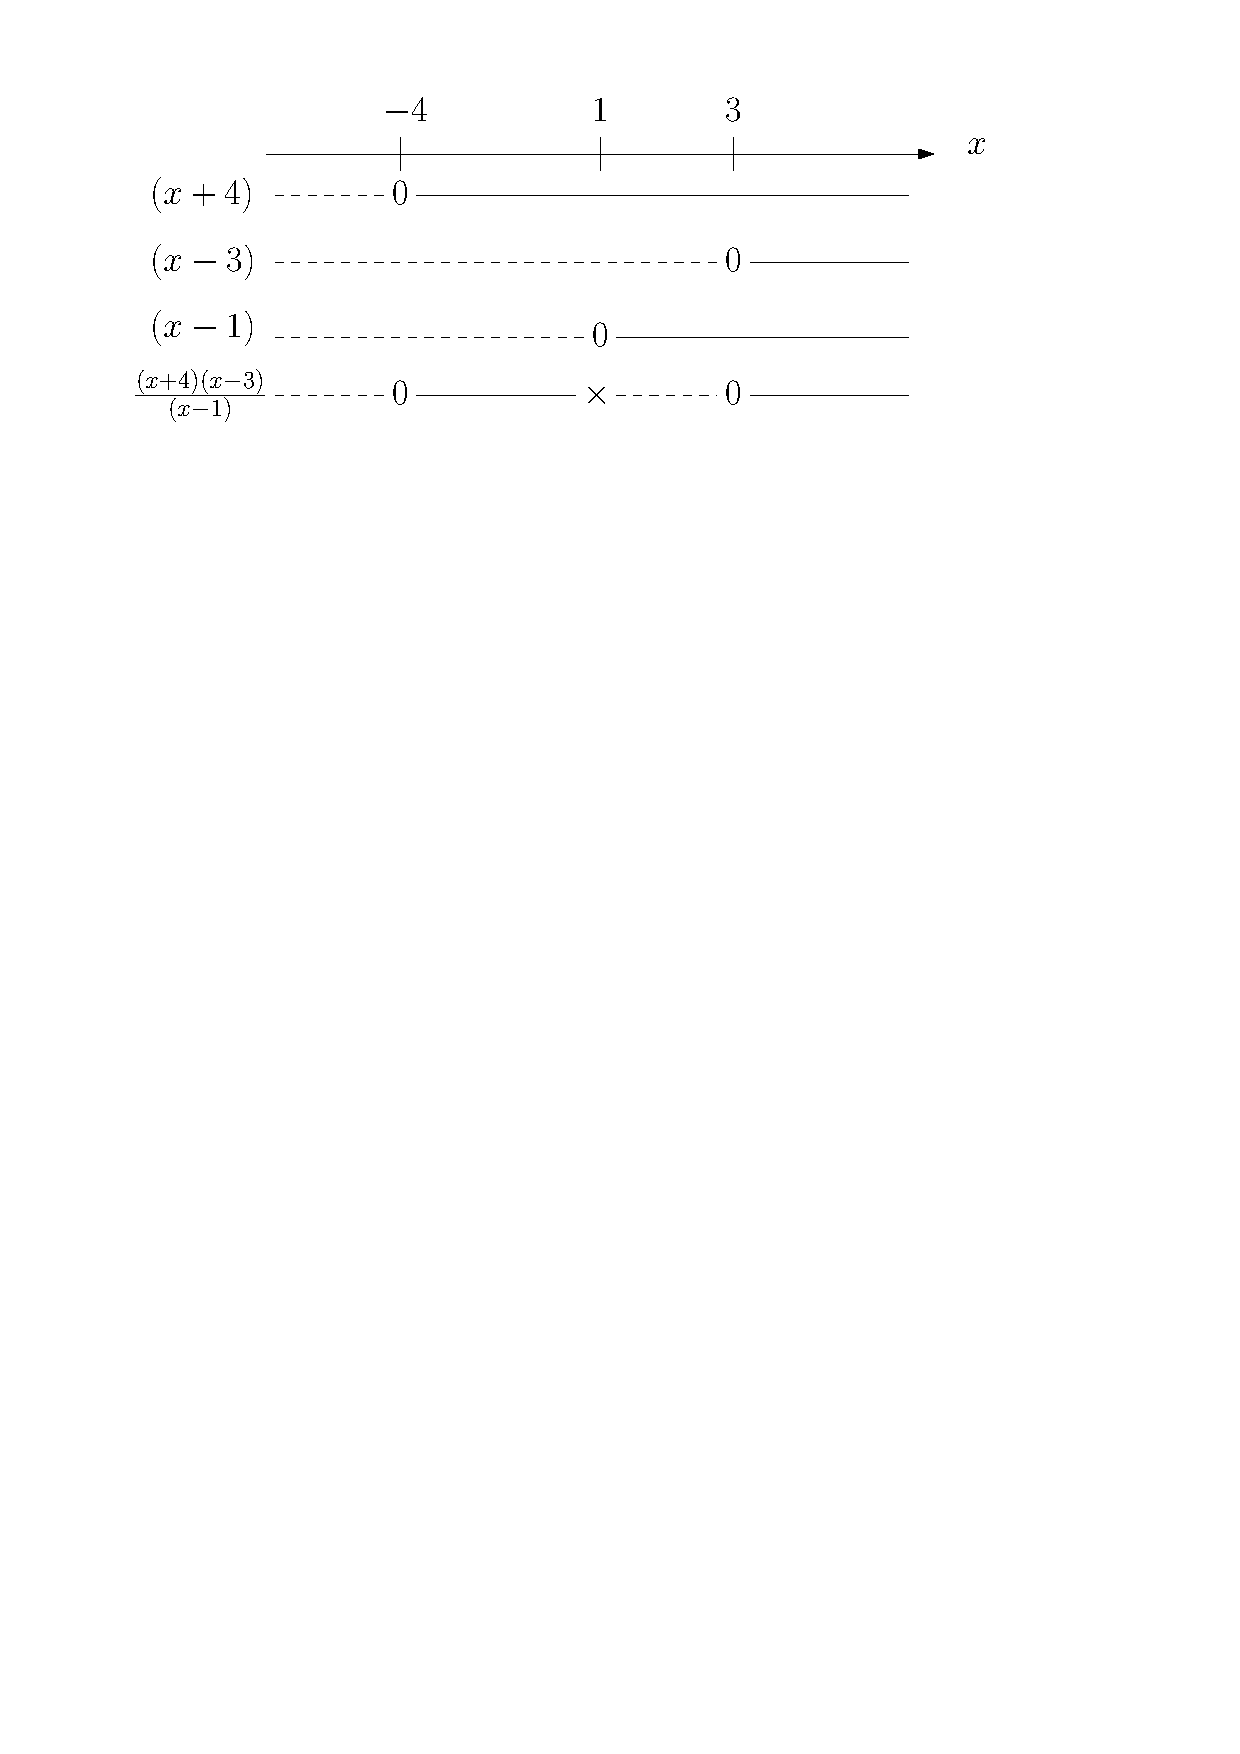
\includegraphics[width=0.85\linewidth]{figs/del1_oppg4c.pdf}
		\label{fig:del1_oppg4c}
	\end{figure}
	
	Vi ser dermed at $$\frac{(x+4)(x-3)}{x-1} \geq 0$$ når \answer{$-4 \leq x < 1$ og når $x \geq 3$}.
	
\end{easylist}

\subsection*{Oppgave 5}

\begin{easylist}[enumerate]
	\ListProperties(Style2*=,Numbers=a,Numbers1=l,FinalMark={)})


\end{easylist}


	
\subsection*{Oppgave 6}

\begin{easylist}[enumerate]
	\ListProperties(Style2*=,Numbers=a,Numbers1=l,FinalMark={)})
	
	# Vi finner nullpunktene til en funksjon ved å sette funksjonsuttrykket lik $0$: $f(x) = 0$, og løser likningen.
	
	\begin{equation*}
	\begin{aligned}
		e^{2x} - 4e^{x} + 3 &= 0 \qquad \textnormal{vi setter $e^x = u$}\\ 
		u^2 - 4u + 3 &= 0\\	
	\end{aligned}
	\end{equation*}
	
	Vi bruker abc-formelen for å løse denne andregradslikningen, og får at $u = 3$ og $u = 1$. Dette gir oss to likninger som vi nå kan løse for $x$.
	
	\begin{equation*}
		\begin{aligned}
		u = 3 & \qquad u = 1 \\
		e^x = 3 & \qquad e^x = 1 \\
		\ln e^x = \ln 1 & \qquad \ln e^x = \ln 3\\
		x = 0 & \qquad x = \ln 3 \approx 1.10
		\end{aligned}
	\end{equation*}
	
	Nullpunktene til $f(x)$ er altså $	\answer{x = 0}$ og $\answer{x = \ln 3 \approx 1.10}$.
	
	# For å bestemme eventuelle topp- og bunnpunkter til funksjonen, deriverer vi funksjonen og ser når den deriverte er lik $0$. Det er blant løsningene vi får til $f'(x) = 0$, vi vil finne de eventuelle topp- og bunnpunktene.
	
	\begin{equation*}
		\begin{aligned}
		f'(x) &= 2e^{2x} - 4e^x \\
		& = 2e^x(e^x - 2)
		\end{aligned}
	\end{equation*}
	
	Så løser vi likningen $f'(x) = 0$
	
	\begin{equation*}
		\begin{aligned}
		f'(x) & = 0 \\
		2e^x(e^x - 2) & = 0 \qquad \textnormal{$2e^x > 0$ alltid, så vi får}\\
		e^x - 2 & = 0 \\
		e^x & = 2 \\
		\ln e^x &=  \ln 2\\
		x & = \ln 2
		\end{aligned}
	\end{equation*}
	
	Vi lager fortegnslinje for å sjekke om dette punktet er et topp- eller bunnpunkt, eller ingen av delene.
	
	\begin{figure}[ht!]
		\centering
		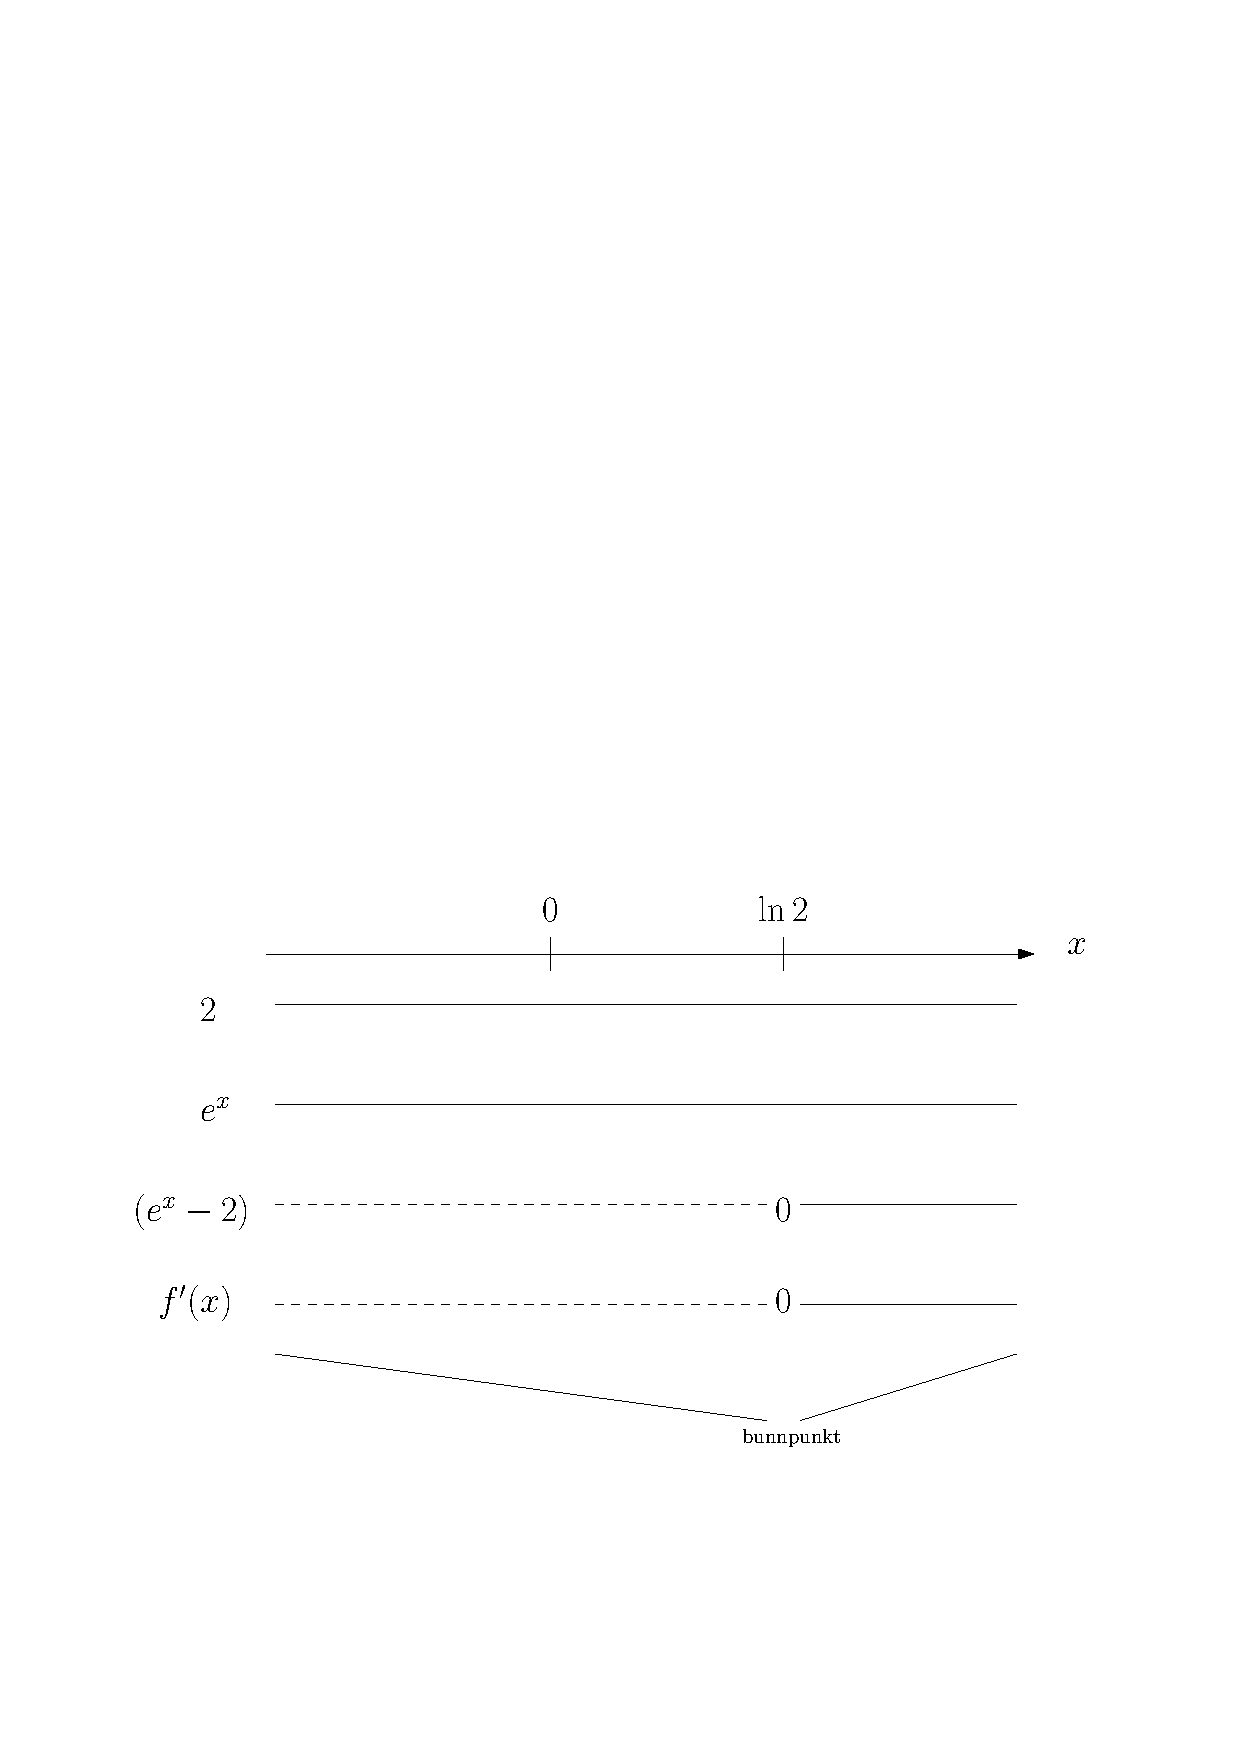
\includegraphics[width=0.85\linewidth]{figs/del1_oppg6b.pdf}
		\label{fig:del1_oppg6b}
	\end{figure}
	
	Vi ser av fortegnslinjen at vi har et bunnpunkt i $x = \ln 2$. Funksjonsverdien for denne $x$-verdien er
	
	\begin{equation*}
		\begin{aligned}
		f(\ln 2) & = e^{2\ln2} - 4e^{\ln 2} + 3\\
		& = e^{\ln 2^2} - 4e^{\ln 2} + 3 \\
		& = 4 - 8 + 3 \\
		& = -1
		\end{aligned}
	\end{equation*}
	
	Bunnpunktet er altså $\answer{(\ln 2, -1)}$.
	
	
	# Når vi skal bestemme eventuelle vendepunkt, kan vi undersøke hvor den dobbeltderiverte av funksjonen endrer fortegn. Vi deriverer derfor den deriverte vi fant i forrige deloppgave. 
	
	\begin{equation*}
		\begin{aligned}
		f''(x) & = 4e^{2x} - 4e^x \\
		& = 4e^x(e^x -1)
		\end{aligned}
	\end{equation*}
	
	Deretter setter vi den dobbeltderiverte lik $0$, og lager igjen fortegnslinje som i oppgaven over.
	
	\begin{equation*}
		\begin{aligned}
		f''(x) & = 0 \\
		4e^x(e^x-1) & = 0 \qquad \textnormal{$4e^x > 0$ alltid, så vi får}\\ 
		e^x -1 & = 0 \\
		e^x & = 1 \\
		\ln e^x & = \ln 1 \\
		x & = 0
		\end{aligned}
	\end{equation*}
	
	Fortegnslinjen vil se slik ut:
	
	\begin{figure}[ht!]
		\centering
		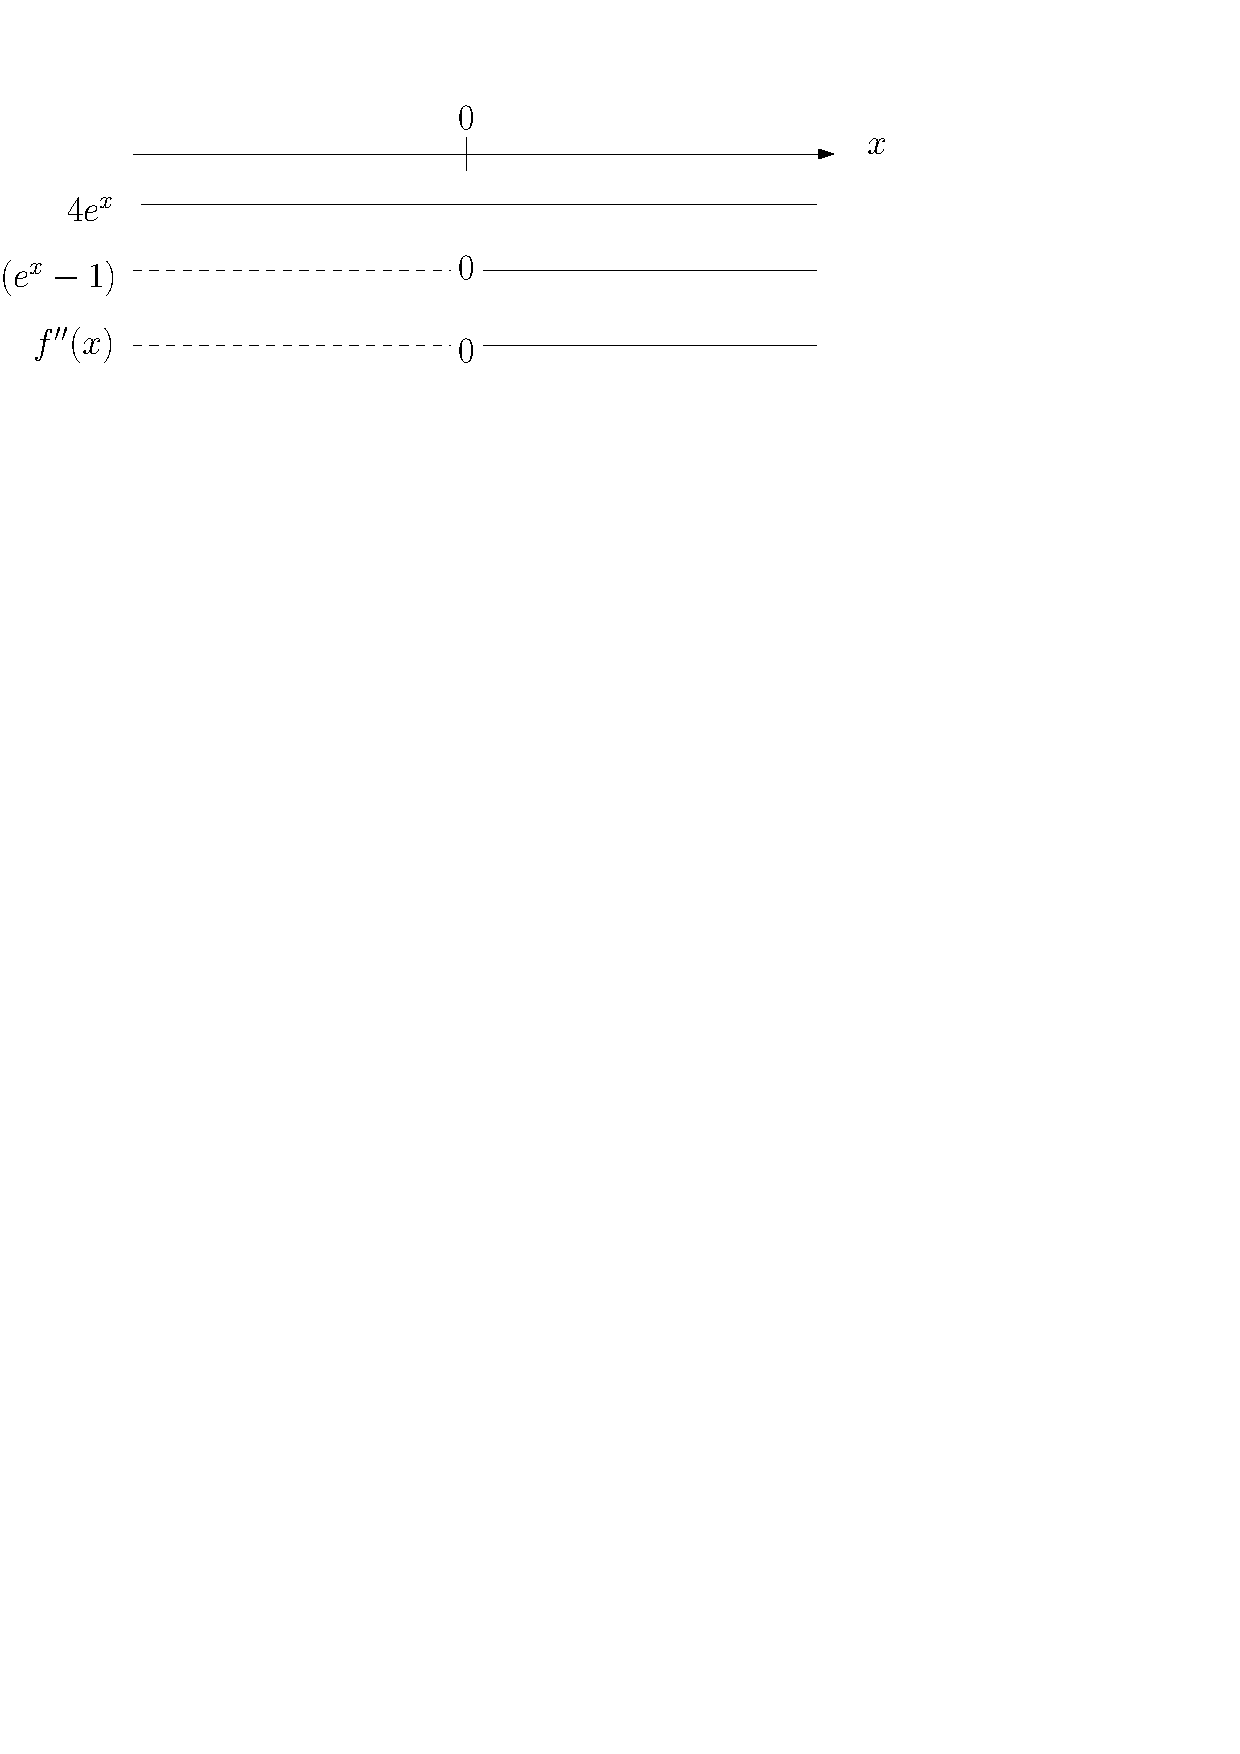
\includegraphics[width=0.85\linewidth]{figs/del1_oppg6c.pdf}
		\label{fig:del1_oppg6c}
	\end{figure}
	
	Vi ser altså at den dobbeltderiverte skifter fortegn når $x=0$. Den tilhørende funksjonsverdien er: 
	
	\begin{equation*}
	\begin{aligned}
	f(0) & = e^{2 \cdot 0} - 4e^0 + 3\\
	& = 1 -4 +3\\
	& = 0\\
	\end{aligned}
	\end{equation*}	
	
	Vendepunktet for funksjonen er altså i punktet $\answer{(0,0)}$.
	
	# Når vi lager en skisse av grafen til funksjonen, er det veldig lurt å tegne inn de punktene vi har funnet i oppgavene over. Disse punktene gir oss god informasjon om hvordan grafen omtrent kan se ut. 
	
	\begin{figure}[ht!]
		\centering
		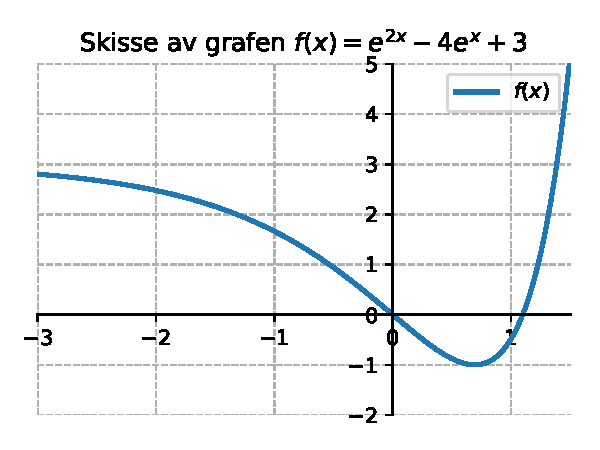
\includegraphics[width = 0.85\linewidth]{figs/del1_oppg6d.pdf}
		\label{fig:del1_oppg6d}
	\end{figure}
	
\end{easylist}

\subsection*{Oppgave 7}

\begin{easylist}[enumerate]
	\ListProperties(Style2*=,Numbers=a,Numbers1=l,FinalMark={)})
	
	# En måte å vise at trekantene er formlike på, er å sjekke at forholdet mellom samsvarende sider er det samme. 
	
	\begin{figure}[ht!]
		\centering
		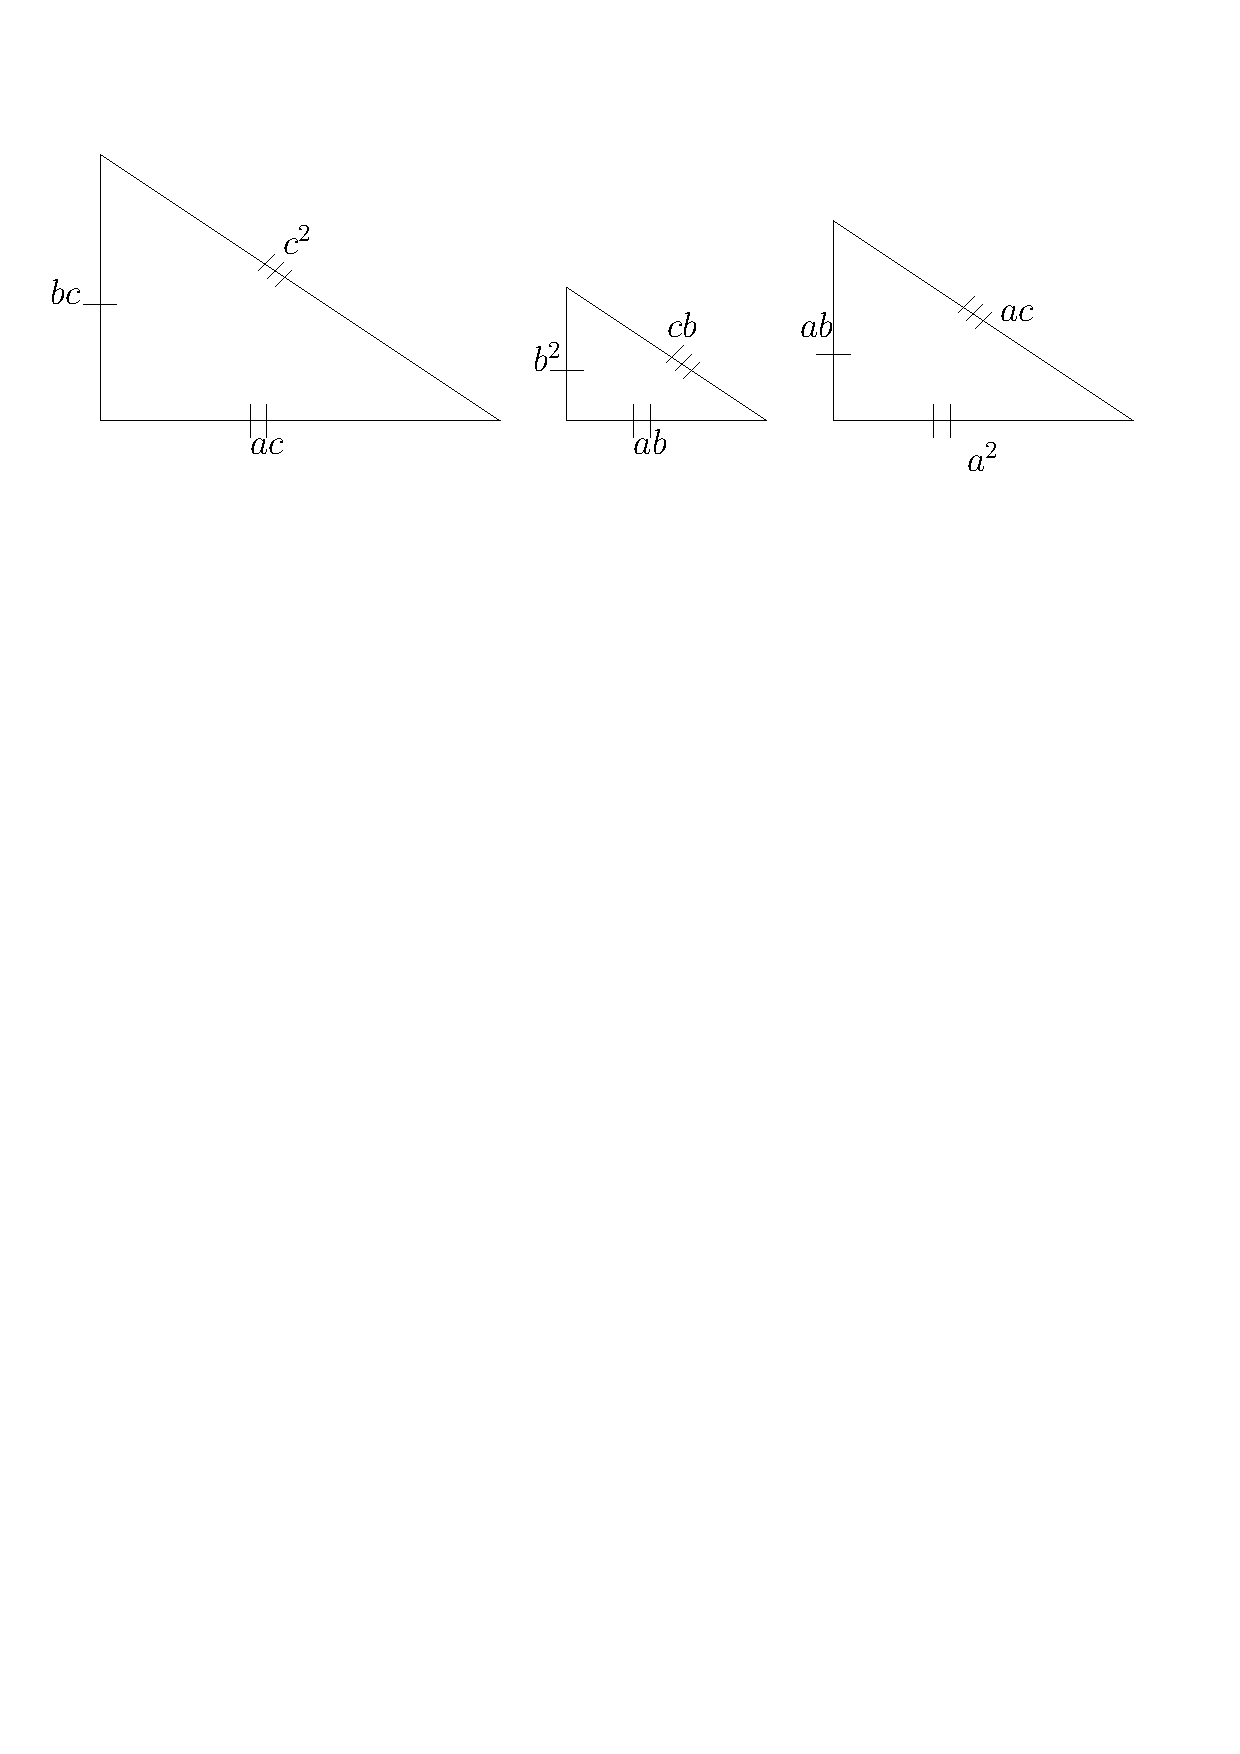
\includegraphics[width = 0.85\linewidth]{figs/del1_oppg7.pdf}
		\label{fig:del1_oppg7}
	\end{figure}	
	
		Vi starter med å vise at trekant 1 og 2 er formlike. Forholdet mellom de formlike sidene er:
		
	
	\begin{equation*}
		\begin{aligned}
			\frac{bc}{b^2} & = \frac{c}{b} \\
			\frac{ac}{ab} & = \frac{c}{b} \\
			\frac{c^2}{cb} & = \frac{c}{b} \\			
		\end{aligned}
	\end{equation*}
	
	Deretter sjekker vi om trekant 2 og 3 er formlike
	
	\begin{equation*}
	\begin{aligned}
	\frac{b^2}{ab} & = \frac{b}{a} \\
	\frac{ab}{a^2} & = \frac{b}{a} \\
	\frac{cb}{ac} & = \frac{b}{a} \\			
	\end{aligned}
	\end{equation*}
	
	Vi ser altså at trekant 1 er formlik med trekant 2 og at trekant 2 er formlik med trekant 3. Da må også trekant 1 og 3 være formlike. 
	
	# For å vise at punktene E, D og C ligger på en rett linje, må vi vise at $\angle ADE + \angle BDC = \ang{180} $. Siden de tre trekantene er formlike, vet vi at samsvarende vinkler er like store. Vi vet også at $\angle ADB = \ang{90}$, så det gjenstår å vise at $\angle ADE + \angle BDC = \ang{90}$.
	
	Dette gjør vi ved å trekke to hjelpelinjer som vist på figuren nedenfor. Vi vet at to parallelle linjer som skjæres av samme linje danner samsvarende vinkler. I tillegg får vi toppvinkler. Derfor vet vi at $\angle BAD$ er samsvarende vinkel med $\angle ADE$, som vil si at disse to vinklene er like store. Vi får samme tilfelle for $\angle ABD$. Denne er samsvarende med vinkel $\angle BDC$, altså er disse to vinklene også like store.
	
	%Legg til figur
	
	Siden summen av vinklene i en trekant er $180$, vet vi at $\angle BAD + \angle  ABD ? \ang{90}$, og dermed vet vi også at $\angle ADE + \angle BDC = \ang{90}$. Vi har da at $\angle EDC  = \ang{180}$, og dermed må punktene E, D og C ligge på samme linje.
	
	# Fra oppgaven over har vi at $\angle DAE + \angle BAD = \ang{90}$ og at $\angle DBA + \angle CBD = \ang{90}$. Da har vi at alle hjørnene i firkanten vår er $\ang{90}$, altså har vi et rektangel. 
	
	I et rektangel vet vi at parallelle sider er like lange, det vil si at lengden av siden EC skal være lik lengden av siden AB. Altså: $a^2 + b^2 = c^2$, som er Pytagoras' setning.
	
\end{easylist}
\newpage


\section*{Del 2 - med hjelpemidler}

\subsection*{Oppgave 1}

\subsection*{Oppgave 2}

\begin{easylist}[enumerate]
	\ListProperties(Style2*=,Numbers=a,Numbers1=l,FinalMark={)})

	Likningen for en sirkel kan skrives $$x^2 + y^2 + ax + by + c = 0$$, og vi får oppgitt at $A(3,8)$, $B(9,6)$ og $C(13,-2)$ ligger på sirkelperiferien. 
	
	# For at likningen skal gjelde for en sirkel som går gjennom alle de gitte punktene, må likningen gå opp uansett hvilket punkt vi setter inn i likningen. For å finne et likningssystem som svarer til det over, setter vi altså inn $x$- og $y$-koordinatene for hvert av punktene i hver sin likning. Likningssystemet blir da:
	
	\begin{equation*}
		\begin{cases} 3^2 + 8^2 + 3a + 8b + c = 0
		\\ 9^2 + 6^2 + 9a + 6b + c = 0 
		\\ 13^2 + (-2)^2 + 13a - 2b + c = 0 
		\end{cases}
	\end{equation*}
	
	# Vi skriver inn hver likning i CAS, markerer alle linjene og trykker på x=. Vi kan også bruke kommandoen Løs, og skrive inn hvilke linjer CAS skal løse. Dette ville vi i mitt tilfelle gjort slik: Løs(\{\$1,\$2,\$3\}).

	\begin{figure}[ht!]
		\centering
		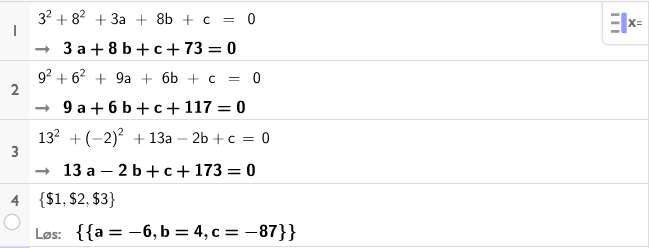
\includegraphics[width = 0.85\linewidth]{figs/del2_oppg2.png}
		\label{fig:del1_oppg7}
	\end{figure}

\end{easylist}


\subsection*{Oppgave 3}




\end{document}